\documentclass[10pt]{extarticle}
\title{}
\author{Avinash Iyer}
\date{}
\usepackage[shortlabels]{enumitem}

%font setup
%
%\usepackage{newpxtext,eulerpx}

%paper setup
\usepackage{geometry}
\geometry{letterpaper, portrait, margin=1in}
\usepackage{fancyhdr}

%symbols
\usepackage{amsmath}
\usepackage{amssymb}
\usepackage{mathtools}
\usepackage{hyperref}
\usepackage{gensymb}

\usepackage[T1]{fontenc}
\usepackage[utf8]{inputenc}

%chemistry stuff
\usepackage[version=4]{mhchem}
\usepackage{chemfig}

%plotting
\usepackage{pgfplots}
\usepackage{tikz}
\tikzset{middleweight/.style={pos = 0.5, fill=white}}
\tikzset{weight/.style={pos = 0.5, fill = white}}
\tikzset{lateweight/.style={pos = 0.75, fill = white}}
\tikzset{earlyweight/.style={pos = 0.25, fill=white}}

%\usepackage{natbib}

%graphics stuff
\usepackage{graphicx}
\graphicspath{ {./images/} }

%code stuff
%when using minted, make sure to add the -shell-escape flag
%you can use lstlisting if you don't want to use minted
%\usepackage{minted}
%\usemintedstyle{pastie}
%\newminted[javacode]{java}{frame=lines,framesep=2mm,linenos=true,fontsize=\footnotesize,tabsize=3,autogobble,}
%\newminted[cppcode]{cpp}{frame=lines,framesep=2mm,linenos=true,fontsize=\footnotesize,tabsize=3,autogobble,}

\usepackage{listings}
\usepackage{color}
\definecolor{dkgreen}{rgb}{0,0.6,0}
\definecolor{gray}{rgb}{0.5,0.5,0.5}
\definecolor{mauve}{rgb}{0.58,0,0.82}

\lstset{frame=tb,
	language=Java,
	aboveskip=3mm,
	belowskip=3mm,
	showstringspaces=false,
	columns=flexible,
	basicstyle={\small\ttfamily},
	numbers=none,
	numberstyle=\tiny\color{gray},
	keywordstyle=\color{blue},
	commentstyle=\color{dkgreen},
	stringstyle=\color{mauve},
	breaklines=true,
	breakatwhitespace=true,
	tabsize=3
}
% text + color boxes
\usepackage[most]{tcolorbox}
\tcbuselibrary{breakable}
\newtcolorbox{problem}[1]{colback = white, title = {#1}, breakable}
\newtcolorbox{solution}{colback = white, colframe = black!75!white, title = Solution, breakable}
%including PDFs
\usepackage{pdfpages}
\setlength{\parindent}{0pt}

\pagestyle{fancy}
\fancyhf{}
\rhead{Avinash Iyer}
\lhead{Math 400: Class Notes}
\begin{document}{
  \begin{problem}{Graphs and the Three Utilities Problem}
    We can imagine trying to connect three houses below with three utilities without the utility lines crossing.
    \begin{center}
      \includegraphics[width=10cm]{3_utilities_problem_blank}
    \end{center}
    This problem is akin to the graph $K_{3,3}$ (the complete bipartite graph with three vertices in each partite set). 
    \begin{center}
      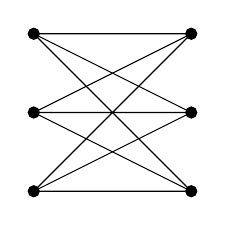
\begin{tikzpicture}
        \filldraw (-1,0) circle (2pt)
              (-1,1) circle (2pt)
              (-1,-1) circle (2pt)
              (1,0) circle (2pt)
              (1,1) circle (2pt)
              (1,-1) circle (2pt);
        \draw (-1,0) -- (1,0) -- (-1,1) -- (1,1) -- (-1,-1) -- (1,-1) -- (-1,0);
        \draw (1,-1) -- (-1,1);
        \draw (1,1) -- (-1,0);
        \draw (1,0) -- (-1,-1);
      \end{tikzpicture}
    \end{center}
    A \textit{graph} is an ordered pair of sets $(V,E)$, where $E\subseteq V\times V$.\\

    For example, if $V = \{a,b,c\}$ and $E = \{(a,b),(a,c)\}$, then $(V,E)$ is a graph. The goal of the three utilities puzzle is to draw $K_{3,3}$ in $\mathbb{R}^2$ without any edges crossing. A graph that can be drawn as such is \textit{planar}.
    \begin{itemize}
      \item $K_{3,3}$ is not planar.
      \item $K_{2,4}$ is planar.
    \end{itemize}
    \begin{center}
      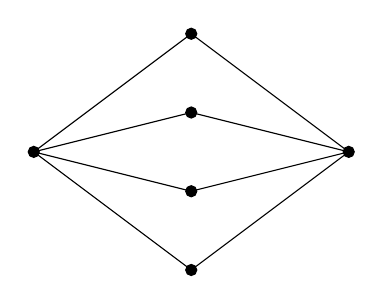
\begin{tikzpicture}
        \filldraw (-2,0) circle (2pt)
                  (2,0) circle (2pt)
                  (0,0.5) circle (2pt)
                  (0,1.5) circle (2pt)
                  (0,-0.5) circle (2pt)
                  (0,-1.5) circle (2pt);
        \draw (-2,0) -- (0,1.5);
        \draw (-2,0) -- (0,-1.5);
        \draw (-2,0) -- (0,0.5);
        \draw (-2,0) -- (0,-0.5);
        \draw (2,0) -- (0,1.5);
        \draw (2,0) -- (0,-1.5);
        \draw (2,0) -- (0,0.5);
        \draw (2,0) -- (0,-0.5);
      \end{tikzpicture}
    \end{center}
    \begin{problem}{Euler's Theorem}
      Let $G\subseteq \mathbb{R}^2$ be a planar graph (i.e., drawn in $\mathbb{R}^2$ without edge crossings). Each disjoint subset of $\mathbb{R}^2-G$ is a \textit{face} of G.\\

      For every graph $G$ embedded in $\mathbb{R}^2$ (i.e., drawn without edge crossings) with $V$ vertices, $E$ edges, and $F$ faces, the following is true:
      \[
        V-E+F = 2
      \]
    \end{problem}
    We will use this theorem to show that you cannot connect the three houses to the three utilities as follows:
    \begin{problem}{Outline Proof (of $K_{3,3}$'s non-planarity)}
      Suppose toward contradiction that $K_{3,3}$ is planar. Then, by Euler's Theorem, we know that $V-E+F = 2$.\\

      We know that $K_{3,3}$ has six vertices and nine edges, so we know that $6-9+F = 2$. Therefore, we know that there must be $5$ faces. In order to enclose a face, there must be at least four edges in $K_{3,3}$ (as there is no edge between two members of a partite set). Additionally, each edge encloses two faces. Therefore, $E\geq 2F$. However, since $E = 9$, and we assume that $F\geq 5$, we have reached a contradiction (as $9<10$). Thus, $K_{3,3}$ is not planar.
    \end{problem}
    \begin{problem}{Four-Color Theorem}
      Every planar graph can be colored (adjacent vertices do not have the same color) with four colors. The planar graph can be colored by fewer colors.
    \end{problem}
    \begin{problem}{Polynomial Example}
      Let $p(a,b,c,d) = ab + ac + ad + bc +bd + cd$. When we factor, we get $p(a,b,c,d) = a(b+c+d) + b(c+d) + cd$. In the first equation, we had to carry out 6 multiplications, while in the second equation we only had to carry out 3 multiplications. We could factor differently:
      \begin{align*}
        p(a,b,c,d) &= ab + ac + ad + bc + bd + cd \\
                   &= a(b+c+d) + b(c+d) + cd\\
                   &= (a+b)(c+d) + ab + cd
      \end{align*}
      We have a lower bound of three multiplications to carry out.\\

      In the arbitrary case, we have the following. We want to find the lowest number of multiplications.
      \begin{align*}
        p(x_1,\dots,x_n) &= \sum_{i = 1}^{n-1}\sum_{j = i+1}^{n} x_ix_j
      \end{align*}
      \tcblower
      The minimum number of multiplications we can do is $n-1$. We can find this via a graph with $n$ vertices $\{x_1,\dots,x_n\}$, and for $x_ix_j$ in $p$, we have an edge from $x_i$ to $x_j$. This is the complete graph on $n$ vertices, $K_n$. Each complete bipartite subgraph represents a multiplication — so our question can be restated as follows:
      \begin{quote}
          Given a complete graph on $n$ vertices, $K_n$, partition its edges into as few complete graphs as possible.
      \end{quote}
      The answer for this is $n-1$, with a proof in linear algebra. However, there is no graph theory-specific proof for this question.
    \end{problem}
  \end{problem}
  \begin{problem}{Light Cycles}
    \begin{tcbraster}[raster columns = 1,colframe = black!75!white,colback=white]
      \tcbincludepdf{images/road_problem.pdf}
    \end{tcbraster}
  \end{problem}
  \begin{problem}{Diestel book: Overview}
    A \textbf{graph} is an ordered pair $G = (V,E)$ of sets such that $\forall e\in E,~e=\{v,w\}$ for some $v,w\in V$.
    \begin{problem}{Paths and Cycles}
      A graph $H$ is a \textbf{subgraph} of a graph $G$ if $V(H) \subseteq V(G)$ and $E(H) \subseteq E(G)$. \\

      A \textbf{path} is a subgraph $P$ of $G$ such that $V(P) = \{v_0,\dots,v_k\}$ and $E(P) = \{v_0v_1,\dots,v_{k-1}v_k\}$. We say the \textbf{length} of $P$ is equal to $|E(P)|$.\\

      If $v_kv_0\in E(G)$, then $C = P + v_kv_0$ is a \textbf{cycle}. $V(C) = V(P)$ and $E(C) = E(P) \cup \{v_0v_k\}$.\\

      \textbf{Abbreviations}: $P = v_0\dots v_k$, and $C = v_0\dots v_kv_0$
    \end{problem}
    \begin{problem}{Degree, Order, and Size}
      Given $v\in V(G)$, the \textbf{degree} of $v$ $d(v) = |\{vw \mid v\in E(G)\}|$. The edge $vw$ is \textbf{incident} to $v$.\\

      The \textbf{order} of $G$ is $|V(G)|$, or $|G|$, and the \textbf{size} of $G$ is $|E(G)|$, or $||G||$.
    \end{problem}
    \begin{problem}{Hamiltonian Cycles}
      A cycle $C\subseteq G$ is \textbf{Hamiltonian} if $V(C) = V(G)$. A graph is Hamiltonian if it contains a Hamiltonian cycle.
      \begin{center}
        \includegraphics[width=0.75\textwidth]{hamiltonian}
      \end{center}
      For example, $G_1$ has a Hamiltonian cycle $\{1,2,4,5,6,3,1\}$, while $G_2$ does not have one as the stray vertex cannot be reached without going over an edge.\\

      For example, the Knight's Tour (where you visit every square on a chess board) involves finding a particular kind of Hamiltonian cycle. 
    \end{problem}
    \begin{problem}{Dirac's Theorem}
      If $G$ is a graph of order $\geq 3$ such that every vertex has degree $\geq \left\lceil\frac{|G|}{2}\right\rceil$, then $G$ is Hamiltonian.
      \tcblower
      Let $P$ be a path in $G$ with maximum length (i.e., \textit{a} longest path).
      \textbf{Outline:}
      \begin{description}
        \item[Step 1] Show that $|V(P)| > \frac{|G|}{2}$
        \item[Step 2] Show $\exists C\subseteq G$ such that $V(C) = V(P)$.
        \item[Step 3] Show that $C$ is a Hamiltonian cycle.
      \end{description}
      \begin{description}
        \item[Step 1] Let $P = (v_1,v_2,\dots,v_k)$ be a path in $G$ with maximum length. Suppose toward contradiction that $|P| < n/2$, meaning $k< n/2$. Then, $\nexists v_i$ such that $v_i$ is connected to any of $v_1,\dots,v_k$, or else we would be able to extend $P$. Thus, $\forall v\in \{v_1,\dots,v_k\}$, $v$ is only adjacent to other members in $v_1,\dots,v_k$. However, this means that the maximum value $v$ can take is $k-1$, and since $k < n/2$, this means $k-1 < n/2$, or that $v$ would not satisfy one of the conditions of $G$. $\bot$
        \item[Step 2] Let $P=v_0\dots v_k$. It suffices to show that $\exists j\in \{2,\dots,k\}$ such that $v_1\leftrightarrow v_j$ and $v_{j-1} \leftrightarrow v_k$. Since $P$ has maximum length, $v_1$ has no neighbor outside $P$ (or else $P$ could be extended). Similarly, $v_k$ has no neighbor outside $P$. However, every vertex has degree at least $2$, meaning $v_1$ must have a neighbor in $P$. Suppose toward contradiction that $\nexists j-1$ such that $v_{j-1} \leftrightarrow v_k$. Then, $N = \{v_{2-1},\dots,v_{k-1-1}\}\geq \frac{n}{2}$ are not neighbors of $v_k$. This means $k\leq n$, so $v_k$ has $k-1-N$ neighbors, implying $d(v_k) < \frac{n}{2}$, which is our contradiction.
        \item[Step 3] Let $P$ is a path of maximum length in $G$, and $C$ be a cycle in $G$ such that $V(C) = V(P)$. Suppose toward contradiction that $|P| < n$. Then, $\exists v\in G$ such that $v\notin P$. Since $d(v) \geq \frac{n}{2}$, $v$ is adjacent to at least one vertex $w\in P$ (as there are not enough vertices outside $P$ for $v$ to be adjacent to). Let $C = (v_{i_1},\dots,v_{i_k},v_{i_1})$. WLOG, $v$ is adjacent to $v_{i_1}$. Then, $P' = v,v_{i_1},\dots,v_{i_k}$ is a path that is longer than $P$, which is a contradiction.
      \end{description}
    \end{problem}
    \begin{problem}{Ore's Theorem}
      If $|G| \geq 3$ and $\forall v,w\in V(G)$ where $v \nleftrightarrow w$ and $d(v) + d(w) \geq n$, then $G$ is Hamiltonian.
      \tcblower
      We can use Ore's Theorem to prove Dirac's Theorem.
    \end{problem}
    \begin{problem}{Vertex Deletion}
      Let $v\in G$. Then, $G-v$ is the subgraph of $G$ with vertices $V(G)\setminus \{v\}$, and edges $E(G)\setminus \{vw\mid vw\in E(G)\}$.
    \end{problem}
    \begin{problem}{Theorem 6.4}
      Let $v_1,\dots,v_k\in V(G)$. Then, $G-v_1-v_2-\cdots-v_k$ has at most $k$ components.
      \begin{problem}{Connectedness}
        A graph $G$ is \textbf{connected} if $\forall v,w\in V(G)$, $\exists P: v\dots w$.
      \end{problem}
    \end{problem}
  \end{problem}
  \begin{problem}{Distinct Representatives}
    Suppose we want to pick one student representative from every Oxy math class. No student should be chosen more than once. Say there are $n$ classes: $c_1,\dots,c_n$, where $c_i = \{s_1,\dots,s_{k_i}\}$, where $1\leq i \leq n$.\\

    Obviously, there must be at least $n$ students in all classes combined: i.e.,
    \begin{align*}
      \left|\bigcup c_i\right| &\geq n
    \end{align*}
    However, this goes deeper:
    \begin{align*}
      |c_1 \cup c_2| &\geq 2\\
      |c_3 \cup c_5 \cup c_6| &\geq 3\\
                              &\vdots\\
      |c_{i_1} \cup \cdots \cup c_{i_r}| &\geq r~\forall r\tag*{(*)}
    \end{align*}
    Obviously, condition (*) is necessary.\\

    We want $c_i$ and $c_j$ to be distinct, (even when they are equal as sets).\\

    Let $Z = (c_1,\dots,c_n)$ be a finite sequence. Then, $(c_{i_1},\dots,c_{i_k})$ is a subsequence of $Z$ if $i_1<\dots,i_k$.
    \begin{problem}{Hall's Theorem}
      Let $Z = (c_1,\dots,c_n)$ be a sequence of sets $c_i$. Suppose that for every subsequence $Y$ of $Z$ with $Y = (c_{i_1},\dots,c_{i_k})$ such that $|c_{i_1} \cup \cdots \cup c_{i_k}| \geq k$. Then, $\exists$ pairwise distinct $s_1,\dots,s_n$ with $s_i\in c_i$.
      \begin{description}
        \tiny
        \item[Note] (*) is a sufficient condition
      \end{description}
    \end{problem}
      Informally, we can restate the premise as follows: Let $G$ be a bipartite graph. One set of vertices $c_1,\dots,c_n$, is the classes, and the other set $s_1,\dots,s_m$ is the set of all students. Each vertex $c_i$ is connected by edges to its students.
    \begin{problem}{Hall's Theorem (In Graphs)}
      Let $G$ be a bipartite graph on vertices $C\sqcup S$, where $C = \{c_1,\dots,c_n\}$ and $S = \{s_1,\dots,s_m\}$. Then, $G$ has a matching (i.e., a set of pairwise disjoint edges) if and only if $\forall r~1\leq r\leq n$, any $r$ vertices in $C$ are connected to at least $r$ vertices in $S$.
    \end{problem}
  \end{problem}
}\end{document}
